%************************************************
\chapter{Discussion}\label{ch:discussion}
%************************************************
In this chapter, the learning performance and regularization behavior of the ALIF, STDP-ALIF, and Izhikevich neurons are compared and discussed.
Then, the effect of stacking multiple recurrent layers on the learning performance and speed is examined.
Next, possible future research avenues are discussed.
\section{Results}\label{sec:results}

	Figure \ref{fig:inoutpair} shows a typical classification result of a full validation sentence.

	\begin{figure}[ht]
	    \myfloatalign
	    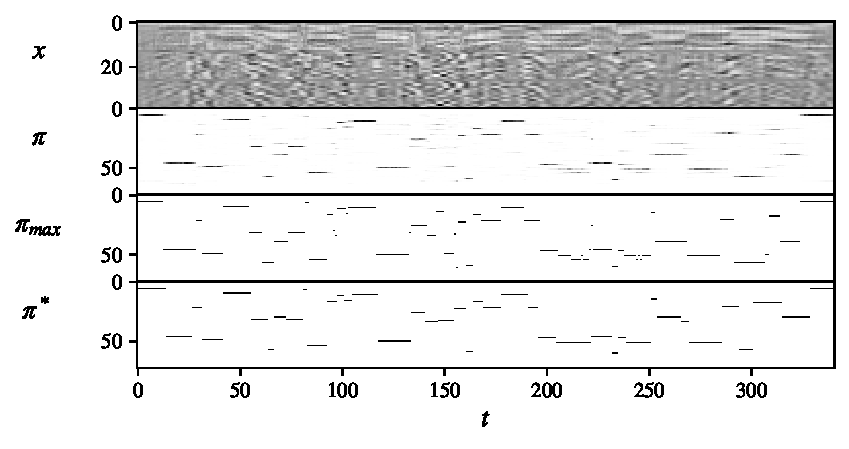
\includegraphics[width=\linewidth]{gfx/InOutPair}
	    \caption[Input/output/target example]{An example validation result using a trained ALIF model. The plot in the top row shows the standardized MFCC frames including its first and second derivatives of a sentence changing over time. The plot in the second row shows the probability distributions $\pi$ of the frame-wise outputs of the model. The plot in the third row indicates the predicted phone $\pi_\text{max}$ per frame. The plot in the last row shows the target phones $\pi^*$.}
	    \label{fig:inoutpair}
	  \end{figure}
	\subsection{Comparing neuron models}

		\paragraph{Accuracy}
			The main outcome of the neuron model comparison is that in these results, the ALIF and STDP-ALIF neuron perform better than the corrected (and default) Izhikevich e-prop neuron model in classifying phones in the TIMIT dataset.
			In Figure \ref{fig:percwrong} the Izhikevich neuron reaches a misclassification rate of 93.8\% on the test set, which is only slightly better than constantly predicting the most frequent class.
			The ALIF neuron model reaches a test misclassification rate of 58.4\% in relatively few iterations, after which validation performance starts to decrease.
			The STDP-ALIF neuron model scores best, reaching a performance of 48.3\% after approximately 3500 iterations, suggesting that the addition of the STDP mechanism to the ALIF neuron improves the classification performance.
			Furthermore, the STDP-ALIF model does not show signs of overfitting as much as the ALIF neuron such as a decreasing validation performance in Figure \ref{fig:percwrong}.
			However, the Izhikevich neuron shows STDP behavior too but performs poorly, suggesting that STDP by itself does not necessarily constitute a well-performing neuron model.
			The STDP-ALIF neuron may instead work by virtue of another factor, such as its better spike frequency adaptation compared to the Izhikevich neuron model.
			Note that the test performance was obtained from the model with the best validation accuracy (the used hyperparameters are listed in Table \ref{tab:hparams}).

			Figure \ref{fig:crossentropy} illustrates the decrease of the cross-entropy score, which for the ALIF and STDP-ALIF neurons is comparable to that of the misclassification rate.
			The cross-entropy and classification performance of the Izhikevich neuron stalls relatively quickly at poor levels, suggesting that it trains its bias toward more frequent phone classes in the training data rather than learning a general relationship between input MFCCs and classes.

			\begin{figure}[bth]
			    \myfloatalign
			    \subfloat[Percentage of samples wrongly classified.]
			    {\label{fig:percwrong}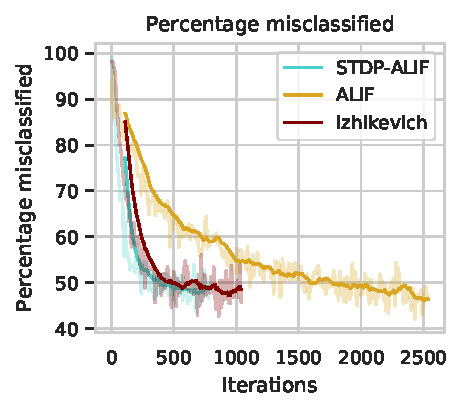
\includegraphics[height=5cm, keepaspectratio]{gfx/percwrong}} \quad
			    \subfloat[Cross-entropy loss (log-scaled).]
			    {\label{fig:crossentropy}%
			        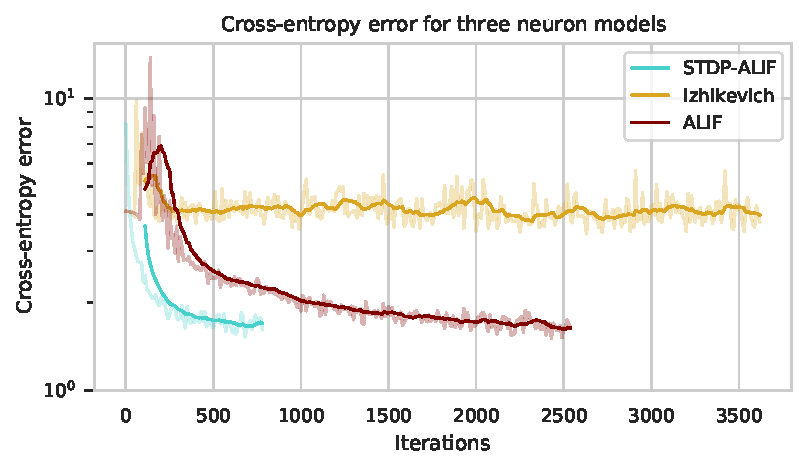
\includegraphics[height=5cm, keepaspectratio]{gfx/crossentropy}}
			    \caption[Single-layer classification performance per neuron model]{Classification performance on the validation data for each of the three neuron models in a single-layer e-prop model. The opaque lines indicate the running average of the real validation scores indicated by the transparent lines. The star symbols indicate the performances on the test set, with a misclassification rate of 93.5\% for the Izhikevich neuron, 58.4\% for the ALIF neuron, and 48.3\% for the STDP-ALIF neuron type.}\label{fig:sl-acc}
			\end{figure}

		\paragraph{Firing rate}
			Figure \ref{fig:freqs} illustrates the effect of the firing regularization term.
			It can be observed that the ALIF and STDP-ALIF neuron models are able to quickly modulate their mean spiking frequencies to the desired target frequency of \SI{10}{\Hz}, but the Izhikevich neuron overshoots to a mean spiking frequency of approximately \SI{18}{\Hz}.

			Figure \ref{fig:regerr} illustrates the decrease of the regularization error.
			The regularization error of the Izhikevich and ALIF neuron models quickly converges to fluctuate around a constant value, whereas that of the STDP-ALIF neuron model continues to decrease over time, even after the mean spiking frequency and classification performance have both converged to a plateau.

			\begin{figure}[bth]
			    \myfloatalign
			    \subfloat[Mean spiking frequency. Note the logarithmic horizontal axis.]
			    {\label{fig:freqs}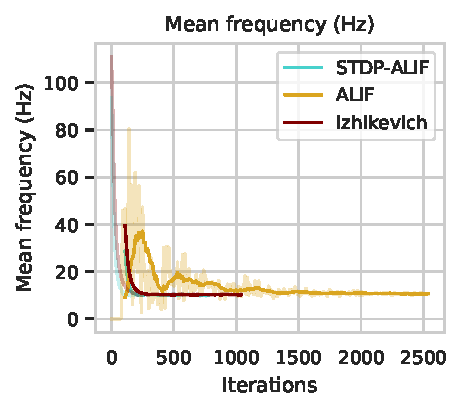
\includegraphics[height=5cm, keepaspectratio]{gfx/hz}} \quad
			    \subfloat[Regularization error. Note the logarithmic vertical axis.]
			    {\label{fig:regerr}%
			        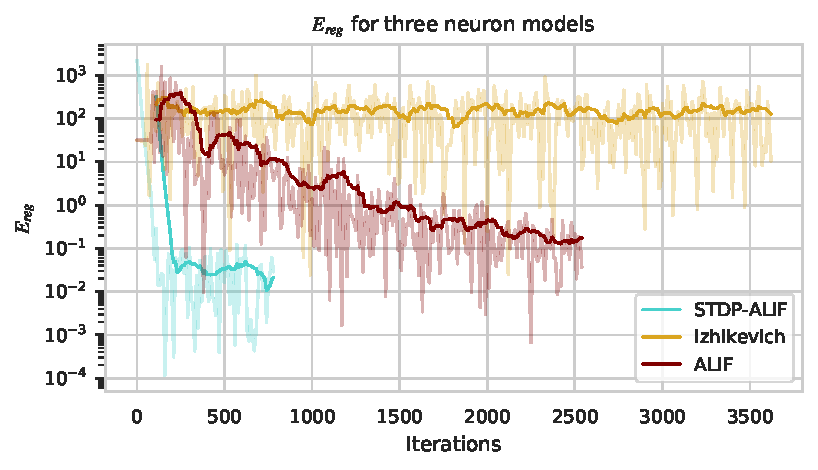
\includegraphics[height=5cm, keepaspectratio]{gfx/regerr}}
			    \caption[Single-layer firing rate regularization per neuron model]{Effect of firing rate regularization on the validation data for each of the three neuron models.}\label{fig:sl-reg}
			\end{figure}

	\subsection{Comparing network depth}
		The comparison between the network depth in Figures \ref{fig:ml-pwrong-alif}--\ref{fig:ml-pwrong-izh} suggests that single-layer e-prop networks train considerably more efficiently and accurately than multi-layer e-prop networks and show less variance among validation runs.
		This holds for all tested neuron types.
		The cross-entropy error, spiking frequency, and regularization error are also better for single-layer networks (see Figure \ref{fig:ml-otherresults}).

		Therefore, rearranging the neurons into a stacked architecture does not appear to improve the classification performance.
		In particular, it appears to diminishes the learning speed to a significant extent and render multi-layer e-prop architectures more inefficient than single-layer ones.
		However, it is not certain that multi-layer architectures are necessarily worse---they train more slowly, but in this report the performance was still improving when their training runs were interrupted due to practical limits.
		Therefore, particularly for the ALIF neuron, the multi-layer networks might outperform the single-layer networks if future work where low computing power and energy costs are not a priority.

		\begin{figure}[bth]
		    \myfloatalign
		    \subfloat[ALIF model.]
		    {\label{fig:ml-pwrong-alif}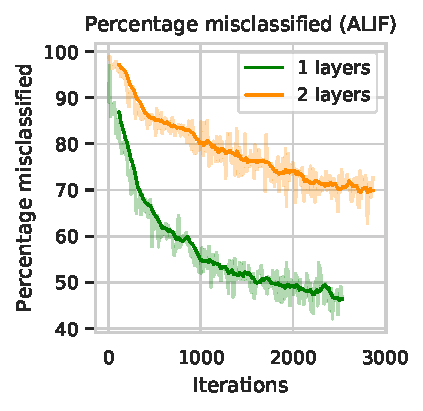
\includegraphics[height=5cm, keepaspectratio]{gfx/ml-percwrong-ALIF}} \quad
		    \subfloat[STDP-ALIF model.]
		    {\label{fig:ml-pwrong-stdpalif}%
		        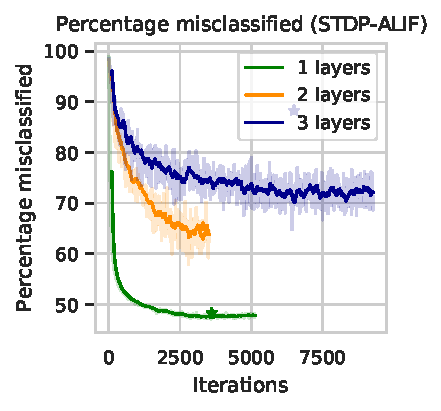
\includegraphics[height=5cm, keepaspectratio]{gfx/ml-percwrong-STDP-ALIF}} \\
		    \subfloat[Izhikevich model.]
		    {\label{fig:ml-pwrong-izh}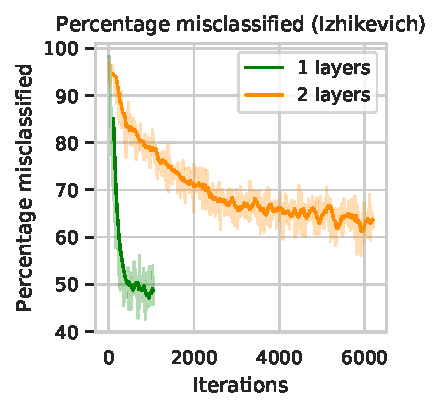
\includegraphics[height=5cm, keepaspectratio]{gfx/ml-percwrong-Izhikevich}}
		    \caption[Single- and multi-layer accuracy comparison]{Accuracy comparison on the validation data between single- and multi-layer e-prop models.}\label{fig:ml-percwrong}
		\end{figure}


\section{Possible improvements}
    There are many hypothetical ways of improving the performance or biological plausibility of e-prop that have not yet been considered in this report.
    For instance, a likely reason that the learning speed of the multi-layer architectures was slower than their single-layer counterparts is that the weights are poorly initialized.
    Empirical observation of the learning process suggested that during early epochs, spiking activity faded in deeper layers, because the spiking activity from a preceding layer is generally weaker than the input values the first layer receives.
    Higher weights in-between layers mitigate this fading activity, but require some search to find a good value.
    In this report, the firing rate regularization term approximated this value, but learning is more efficient with a better initialization, since initial synaptic weights significantly affect the performance of STDP-based SNNs \citep{kim2020initial}.

    Also in this report, certain parameters such as firing rate targets ($f^\text{target}$), activity leak ($\alpha$), and feedback signals were constant for all neurons, except the threshold adaptivity ($\beta$), which was 0 for a randomly selected 25\% of the neurons to emulate non-adaptive LIF neurons.
    Future research could examine the effects of sampling some of these parameters from a distribution for each neuron, thereby creating a more diverse population of neurons with different time scales.
    This sampling requires a careful assessment of the time scales related to the learning task; in particular, the network should be able to process the slowest relevant time scale of the task \citep{jaeger2021dimensions}.
    In the TIMIT classification task, for instance, this could span the whole time fragment, because initial words give semantic context to all subsequent words.
    However, a more predictive time scale for the TIMIT dataset is on the scale of approximately 8 MFCC frames, which is now accurately captured by the adaptive threshold component in the ALIF neuron model.
    Temporal dependencies can also be found when moving in the opposite direction---later words and sounds give informative context to earlier words and sounds.
    In \citet{bellec2020solution}, this context was captured in a bidirectional network, improving the accuracy by nearly 15\%.
    In this report, this was empirically validated as well, but left undiscussed because a bidirectional network is not biologically plausible, as directly accessing future input values violates the ``online'' constraint.
    According to \citet{bellec2020solution}, e-prop suggests that the experimentally found diverse time constants of the firing activity of populations of neurons in different brain areas \citep{runyan2017distinct} are correlated with their capability to handle corresponding ranges of delays in temporal credit assignment for learning.
    Setting different values for these parameters per layer might also have a beneficial effect; \citet{ahmed1998estimates} suggested that deeper layers display slower and weaker adaptation rates than early layers.

    In the brain, neurons primarily tend to connect to nearby neurons.
    This suggests that the effects of the topology within a layer might positively affect the learning process.
    A simple lattice topology might better approximate the connectivity of the brain, decrease the computational complexity in emulations in von Neumann machines, and allow easier on-chip implementations in neuromorphic hardware.
    Hierarchical clustering of neurons might also have a beneficial effect, as this has been demonstrated to improve R-STDP in SNNs \citep{weidel2021unsupervised} and address the scalability issue of SNNs \citep{carrillo2012scalable}.
    Because a neuromorphic system can support complex network operations \citep{hasler1990vlsi}, large-scale conductance-based SNNs \citep{yang2019scalable,Yang2019RealTimeNS} and asynchronous communication in VLSIs through address-event-representation \citep{lazzaro1993silicon,deiss1999pulse} might be suitable to further customize the connectivity graph of an e-prop architecture.

    Other exciting research avenues include connectivity graphs that change over time through a dynamic pruning and growing of weights and neurons.
    Here, the biological motivation is that the human brain prunes synaptic connections during early development \citep{huttenlocher1979synaptic}.
    \citet{elbez2020progressive} demonstrated that 75\% of a SNN can be compressed while preserving its performance, but it is not clear if this can be applied in a biologically plausible way in the e-prop framework.
    However, integrating stochastic synaptic rewiring \citep{kappel2018dynamic} into an ALIF network can improve its short-term memory \citep{bellec2020solution}.

    Finally, synaptic delay might improve the temporal processing power of an e-prop model.
    In this report, communication between neurons was transmitted as a spike over a synapse with a delay of 1 ms.
    This delay could differ among synapses, such that potentially informative past inputs are more accurately preserved in synaptic delays, rather than only in eligibility traces and activity loops.
    This can help deal with tasks that require processing information on multiple time spans \citep{jaeger2021dimensions}.
    This resembles the variable physical length of myelinated biological synapses and the number of nodes of Ranvier along them, affecting the conductance of the action potential \citep{bean2007action}.


\section{Future directions}
    As neuromorphic computing matures, neuroscience improves, and DL increasingly hits fundamental limitations, there is an exciting future for biologically plausible SNNs.
    There is much to gain from cross-fertilization between these fields.
    The popularity of DL was accelerated by accessible platforms to implement and deploy ANNs.
    Similar high-level simulation platforms are now in active development, which can integrate the typical behavior of memristive device models into crossbar architectures within DL systems \citep{lammie2020memtorch}.

    Recent advances in neuromorphic computing indicate this increasing popularity.
    Neuromorphic architectures have been used for mapless navigation with 75 times lower power and better performance \citep{tang2020reinforcement}; as low-power solutions for simultaneous localization and mapping of mobile robots \citep{tang2019spiking}, for planning \citep{fischl2017path}, and control \citep{blum2017neuromorphic}; and self-repairing SNN for fault detection \citep{zhu2017target}.
    While cross-fertilization between neuromorphic computing and quantum computing is starting to take place \citep{russek2016stochastic}, as quantum superposition and entanglement can be used to process information in parallel and in a high-dimensional state space \citep{fujii2017harnessing, yamamoto2017coherent,tacchino2019artificial}, more physics and materials science is required to build efficient neuromorphic architectures \citep{markovic2020physics}.
    The same holds for the cross-fertilization between neuroscience and learning rules of biologically plausible SNNs.
    Nanodevices that emulate biological synapses with learning functions can benefit neuromorphic architectures \citep{yao2017face,wang2018photonic,ren2018analytical}, particularly the two-terminal memristor \citep{jo2010nanoscale,wang2017memristors}.
    However, it has been argued that the learning principles of biological NNs are not explored enough to design engineering solutions \citep{gorban2019unreasonable,taherkhani2018supervised}.
    Feedback connections, for which the brain uses neurotransmitters, may become particularly problematic in large-scale neuromorphic systems.
    Another issue in analog computation is how to match the system's internal temporal processing to that of its inputs.
    Emulating neural dynamics on a physical substrate is more efficient but requires constraints to match the brain's timescales \citep{mead1990neuromorphic,jaeger2021dimensions}.
    Future work on e-prop could explore a combination with attention-based models in order to cover multiple timescales \citep{bellec2020solution}.
